%\documentclass[slide,papersize]{jsarticle}
\documentclass{jsarticle}
\usepackage[dvipdfm]{graphicx,color}
\begin{document}

\date{2012年12月1日}
\title{Metropolis-Hastingsアルゴリズム}
\author{@naoya\_t}
\maketitle

\begin{abstract}
dvi.jsに付けるサンプルを自分で書いてみるテストです。
dvipdfmパッケージを用いた画像の埋め込みにも対応しているので、画像も入れてみました。

内容は Machine Learning Advent Calendar 2012の1日目に投稿したものです。\\
http://qiita.com/items/b9aa110b395d0a5b0b0a
\end{abstract}
\def\naoyat{@naoya\_t}

\section{ご挨拶}

今日から始まりました Machine Learning Advent Calendar 2012 幹事の\naoyat です。

このアドベント・カレンダーの記事内容は、パターン認識・機械学習・自然言語処理・データマイニング等、データサイエンスに関する事でしたら何でもOKです。テーマに沿っていれば分量は問いません。(PRMLの読んだ箇所のまとめ、実装してみた、論文紹介、数式展開、etc.)

執筆する皆さんも読むだけの皆さんも共に楽しみましょう!

\section{さて本題}
いまPRML11章を読んでるので11章から何か。

明日のyag\_aysさんがMCMCあたりと宣言されているので内容がもしかしたら被ってしまうかもしれないけれど、僕はOctaveだしyagさんは多分Rなので良しとしましょう!

\section{Metropolisアルゴリズム}
マルコフ連鎖モンテカルロ(MCMC)において、現在の状態から新しい状態をサンプリングする際、提案分布の対称性
\begin{equation}
q({\bf z}_A|{\bf z}_B)=q({\bf z}_B|{\bf z}_A)
\nonumber\end{equation}
を仮定し、
% \setcounter{equation}{33}
\begin{equation}
\displaystyle A_k({\bf z}^*,{\bf z}^{(\tau)})=min\bigl(1,\frac{\tilde{p}({\bf z}^*)}{\tilde{p}({\bf z}^{(\tau)})}\bigr)
\nonumber\end{equation}
 (11.33) を新しいサンプルを受理するか否かの基準として用いるアルゴリズム。

Metropolisアルゴリズムでは、サンプルが棄却された場合、現在の状態を新しい状態として引き続き用いる。(サンプルが重複することになる)


\newpage
\subsection{図11.9の再現}
図11.9(PRML下巻p.253)では、Metropolisアルゴリズムを用いて2次元ガウス分布からサンプリングする例を図示しています。\\
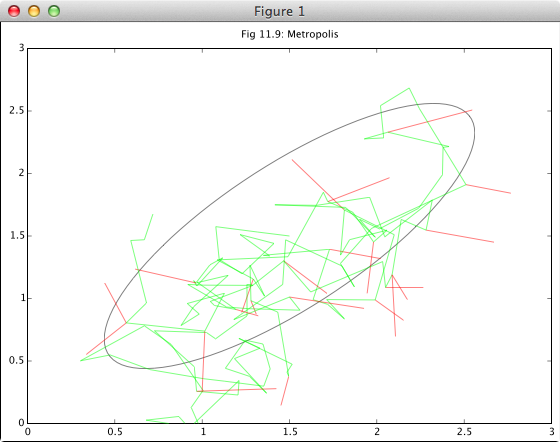
\includegraphics[width=12cm]{img/fig11_9.png}
%[Fig 11.9](http://www1419ue.sakura.ne.jp/prml/11\_2/fig11\_9.png)

\begin{verbatim}
1;
%
% 図11.9 Metropolisアルゴリズムを用いて2次元ガウス分布からサンプリングする例。
%

function plot_gauss2_contour(mu, Sigma)
  cont = zeros(2,101);
  D = chol(Sigma, "lower");
  for j = 1:100
    theta = pi*2/100 * (j-1);
    cont(:,j) = mu + D*[cos(theta); sin(theta)];
  endfor
  cont(:,101) = cont(:,1);
  plot(cont(1,:), cont(2,:), 'k')
endfunction

function pdf = multival_gaussian_pdf(mu, Sigma)
  D = numel(mu);
  Z = ((2*pi)^(D/2)*sqrt(det(Sigma))); % 正規化定数1/Z
  inv_Sigma = inv(Sigma);

  pdf = @(x) 1/Z*exp(-1/2*(x-mu)'*inv_Sigma*(x-mu));
endfunction


mu = [1.5; 1.5];
Sigma = [1.125 0.875; 0.875 1.125]; % λ1=2, v1=[1; 1], λ2=1/4, v2=[1; -1]
p = multival_gaussian_pdf(mu, Sigma);

clf
hold on
axis([0,3,0,3]);
title("Fig 11.9: Metropolis");

plot_gauss2_contour(mu, Sigma);

T = 150;
z = mu;
for j = 1:T
  z_proposal = z + 0.2*randn(2,1);
  A = min(1, p(z_proposal)/p(z)); % (11.33) 受理確率A(z*, z)
  u = rand(1);
  if A > u
    plot([z(1,1) z_proposal(1,1)], [z(2,1) z_proposal(2,1)], 'g')
    z = z_proposal;
  else
    plot([z(1,1) z_proposal(1,1)], [z(2,1) z_proposal(2,1)], 'r')
  endif
endfor

hold off
\end{verbatim}

一般に、等高線は `contour()` でも描けるのですが、図11.9のように標準偏差の線を1本だけ描きたい場合の使い方は分からなかったので、与えられたμとΣから楕円を1つ描く関数 `plot\_gauss2\_contour()` を用意しました。

\section{Metropolis-Hastingsアルゴリズム}
Metropolis-Hastingsアルゴリズム(§11.2.2)は、Metropolisアルゴリズムを提案分布が引数に対して対称な関数でない場合まで一般化したもの。

受理確率 $A_k({\bf z}^*,{\bf z}^{(\tau)})$ の計算が、
式 (11.33)
\begin{equation}
A_k({\bf z}^*,{\bf z}^{(\tau)})=min\bigl(1,\frac{\tilde{p}({\bf z}^*)}{\tilde{p}({\bf z}^{(\tau)})}\bigr)
\end{equation}

から式 (11.44)
\begin{equation}
A_k({\bf z}^*,{\bf z}^{(\tau)})=min\bigl(1,\frac{\tilde{p}({\bf z}^*)q_k({\bf z}^{(\tau)}|{\bf z}^*)}{\tilde{p}({\bf z}^{(\tau)})q_k({\bf z}^*|{\bf z}^{(\tau)})}\bigr)
\end{equation}
に差し替えられている。

\subsection{Metropolis-Hastingアルゴリズムにおいて、提案分布の選択がアルゴリズムの性能に与える影響}

等方ガウス分布を提案分布として用いる場合、標準偏差ρを(サンプリングしたい分布のσに対し)どの程度にしたら良いのかという話。(PRML下巻p.256, 図11.10参照)

\begin{itemize}
\item $\rho << \sigma_{min}$
受理される遷移の割合は高い(9割前後)が、状態空間での前進はゆっくりとしたランダムウォークの形を取り、系列は長い時間にわたって相関を持つことになる。\\
% [mh1](http://www1419ue.sakura.ne.jp/prml/11\_2/mh1.png)
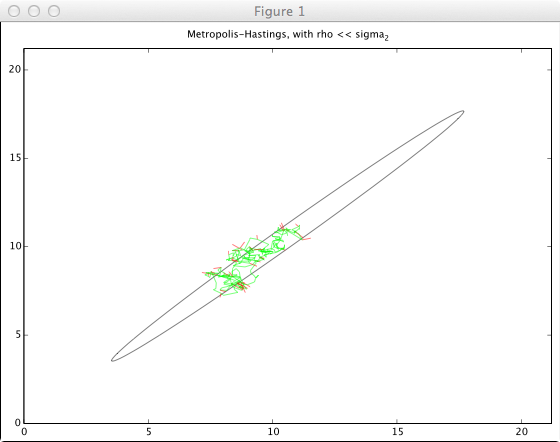
\includegraphics[width=12cm]{img/mh1.png}

\item $\rho=\sigma_{max}$
分散パラメータを大きく取れば、状態空間での前進は大きくなるが、同時に棄却率も高くなる。(この例では受理率7%前後)\\
% [mh3](http://www1419ue.sakura.ne.jp/prml/11\_2/mh3.png)
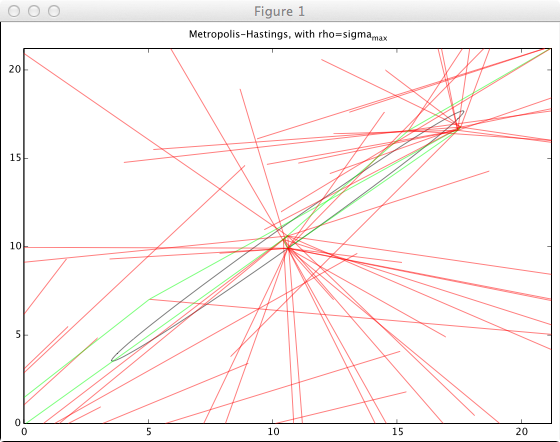
\includegraphics[width=12cm]{img/mh3.png}
\item $\rho=\sigma_{min}$
この位が良いらしい。(受理率7割前後)
ステップ数のオーダーは
\begin{equation}
(\frac{\sigma_{max}}{\sigma_{min}})^2
\end{equation}
になる。\\
% [mh2](http://www1419ue.sakura.ne.jp/prml/11\_2/mh2.png)
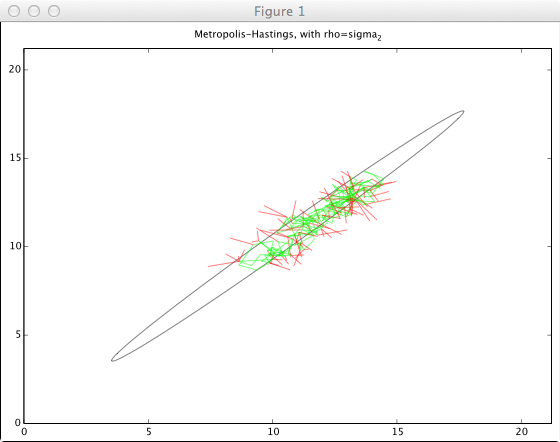
\includegraphics[width=12cm]{img/mh2.png}
\item (おまけ)10ステップ毎にサンプルを採用した場合の散布\\
% [mh9](http://www1419ue.sakura.ne.jp/prml/11\_2/mh9.png)
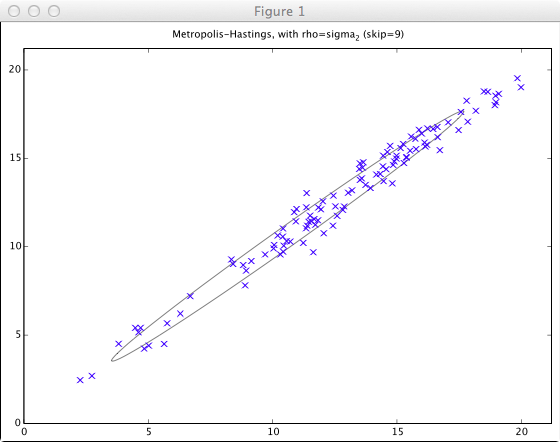
\includegraphics[width=12cm]{img/mh9.png}
\end{itemize}

\begin{verbatim}
1;
%%
%% 図11.9 Metropolisアルゴリズムを用いて2次元ガウス分布からサンプリングする例。
%%

function p = multival_gaussian(x, mu, Sigma)
  D = rows(x);
  dx = x - mu;
  Z = ((2*pi)^(D/2)*sqrt(det(Sigma))); % 正規化定数1/Z
  p = 1/Z*exp(-1/2*dx'*inv(Sigma)*dx);
endfunction

function pdf = multival_gaussian_pdf(mu, Sigma)
  D = numel(mu);
  Z = ((2*pi)^(D/2)*sqrt(det(Sigma))); % 正規化定数1/Z
  inv_Sigma = inv(Sigma);

  pdf = @(x) 1/Z*exp(-1/2*(x-mu)'*inv_Sigma*(x-mu));
endfunction

function plot_gauss2_contour(mu, Sigma, space)
%  [x,y] = meshgrid(space);
%  gauss = multival_gaussian_pdf(mu, Sigma);
%  z = arrayfun(@(x,y)gauss([x;y]), x, y);
%  contour(space,space,z);

  cont = zeros(2,101);
  D = chol(Sigma, "lower");
  for j = 1:100
    theta = pi*2/100 * (j-1);
    cont(:,j) = mu + D*[cos(theta); sin(theta)];
  endfor
  cont(:,101) = cont(:,1);
  plot(cont(1,:), cont(2,:), 'k')
endfunction

global s1 = 10;
global s2 = 0.5;
global mu = [1.5; 1.5]*s1/sqrt(2);
% Sigma = [1.125 0.875; 0.875 1.125]; % λ1=2, v1=[1; 1], λ2=1/4, v2=[1; -1]
H = [1 1; 1 -1]/sqrt(2);
global Sigma = H * [s1*s1 0; 0 s2*s2] * H;
global p = multival_gaussian_pdf(mu, Sigma);

function plot_m(rho, caption, A, line, step=1)
  global s1;
  global s2;
  global mu;
  global Sigma;

  printf("%s: ", caption);

  clf
  hold on
  axis([0,3,0,3]*s1/sqrt(2));
  title(caption);

  plot_gauss2_contour(mu, Sigma);

  T = 150 * step;
  acc = 0;
  z = mu;

  for j = 1:T
    z_proposal = z + rho*randn(2,1);
    p_accept = A(z_proposal, z);
    u = rand(1);
    if p_accept > u
      if line
        plot([z(1,1) z_proposal(1,1)], [z(2,1) z_proposal(2,1)], 'g')
      else
        if mod(j, step) == 0
          plot([z_proposal(1,1)], [z_proposal(2,1)], 'x')
        endif
      endif
      z = z_proposal;
      acc += 1;
    else
      if line
        plot([z(1,1) z_proposal(1,1)], [z(2,1) z_proposal(2,1)], 'r')
      endif
    endif
  endfor

  hold off

  printf("acceptance rate = %g¥n", acc/T);
endfunction


function metropolis(rho, caption, skip=0)
  global p;
  A = @(z_,z) min(1, p(z_)/p(z)); % (11.33)
  plot_m(rho, caption, A, true, 1)
endfunction

function metropolis_hastings(rho, caption, skip=0)
  global p;
  q = @(z_,z) multival_gaussian(z_, z, rho^2*eye(2));
  A = @(z_,z) min(1, (p(z_)*q(z,z_)) / (p(z)*q(z_,z))); % (11.44)
  if skip == 0
    plot_m(rho, caption, A, true, 1)
  else
    plot_m(rho, caption, A, false, 1+skip)
  endif
endfunction


metropolis(0.2, "Metropolis")
pause

metropolis_hastings(0.2, "Metropolis-Hastings, with rho << sigma_2")
pause

metropolis_hastings(s1, "Metropolis-Hastings, with rho=sigma_{max}")
pause

metropolis_hastings(s2, "Metropolis-Hastings, with rho=sigma_2")
pause

metropolis_hastings(s2, "Metropolis-Hastings, with rho=sigma_2 (skip=9)", 9)
\end{verbatim}

\section{終わりに}
告知をいくつか。

\begin{itemize}
\item PRML復々習レーン\#7 http://atnd.org/events/33833 \\
12/15 14:00-20:00 @株式会社VOYAGE GROUP(渋谷・神泉)

\item PRMLカラオケクラスタひみつ集会Vol.1 http://atnd.org/events/33843 \\
12/15 20:30-22:30 @カラオケの鉄人 渋谷道玄坂店 
\end{itemize}

もう1つ。

先月CodeIQで簡単な機械学習(というか線形分類)の問題を出しました。
\begin{itemize}
\item 金貨の真贋を見分けよう https://codeiq.jp/ace/naoyat/q105
\end{itemize}
問題は12/20 10amまで公開していますので、ぜひ挑戦(あるいは秒殺)してみてください!

というわけで明日の担当は @yag\_ays さんです。皆さん乞うご期待!

\end{document}

